\documentclass[10pt, a5paper]{article}
\usepackage{pdfpages}
\usepackage{parallel}
\usepackage[T2A]{fontenc}
\usepackage{ucs}
\usepackage[utf8x]{inputenc}
\usepackage[polish,english,russian]{babel}
\usepackage{hyperref}
\usepackage{rotating}
\usepackage[inner=2cm,top=1.8cm,outer=2cm,bottom=2.3cm,nohead]{geometry}
\usepackage{listings}
\usepackage{graphicx}
\usepackage{wrapfig}
\usepackage{longtable}
\usepackage{indentfirst}
\usepackage{array}
\newcolumntype{P}[1]{>{\raggedright\arraybackslash}p{#1}}
\frenchspacing
\usepackage{fixltx2e} %text sub- and superscripts
\usepackage{icomma} % коскі ў матэматычным рэжыме
\PreloadUnicodePage{4}

\newcommand{\longpage}{\enlargethispage{\baselineskip}}
\newcommand{\shortpage}{\enlargethispage{-\baselineskip}}

\def\switchlang#1{\expandafter\csname switchlang#1\endcsname}
\def\switchlangbe{
\let\saverefname=\refname%
\def\refname{Літаратура}%
\def\figurename{Іл.}%
}
\def\switchlangen{
\let\saverefname=\refname%
\def\refname{References}%
\def\figurename{Fig.}%
}
\def\switchlangru{
\let\saverefname=\refname%
\let\savefigurename=\figurename%
\def\refname{Литература}%
\def\figurename{Рис.}%
}

\hyphenation{admi-ni-stra-tive}
\hyphenation{ex-pe-ri-ence}
\hyphenation{fle-xi-bi-li-ty}
\hyphenation{Py-thon}
\hyphenation{ma-the-ma-ti-cal}
\hyphenation{re-ported}
\hyphenation{imp-le-menta-tions}
\hyphenation{pro-vides}
\hyphenation{en-gi-neering}
\hyphenation{com-pa-ti-bi-li-ty}
\hyphenation{im-pos-sible}
\hyphenation{desk-top}
\hyphenation{elec-tro-nic}
\hyphenation{com-pa-ny}
\hyphenation{de-ve-lop-ment}
\hyphenation{de-ve-loping}
\hyphenation{de-ve-lop}
\hyphenation{da-ta-ba-se}
\hyphenation{plat-forms}
\hyphenation{or-ga-ni-za-tion}
\hyphenation{pro-gramming}
\hyphenation{in-stru-ments}
\hyphenation{Li-nux}
\hyphenation{sour-ce}
\hyphenation{en-vi-ron-ment}
\hyphenation{Te-le-pathy}
\hyphenation{Li-nux-ov-ka}
\hyphenation{Open-BSD}
\hyphenation{Free-BSD}
\hyphenation{men-ti-on-ed}
\hyphenation{app-li-ca-tion}

\def\progref!#1!{\texttt{#1}}
\renewcommand{\arraystretch}{2} %Іначай формулы ў матрыцы зліпаюцца з лініямі
\usepackage{array}

\def\interview #1 (#2), #3, #4, #5\par{

\section[#1, #3, #4]{#1 -- #3, #4}
\def\qname{LVEE}
\def\aname{#1}
\def\q ##1\par{{\noindent \bf \qname: ##1 }\par}
\def\a{{\noindent \bf \aname: } \def\qname{L}\def\aname{#2}}
}

\def\interview* #1 (#2), #3, #4, #5\par{

\section*{#1\\{\small\rm #3, #4. #5}}

\def\qname{LVEE}
\def\aname{#1}
\def\q ##1\par{{\noindent \bf \qname: ##1 }\par}
\def\a{{\noindent \bf \aname: } \def\qname{L}\def\aname{#2}}
}

\switchlang{ru}
\begin{document}
\title{Картографический сервис на OpenSource - доступная картография каждому}
\author{Дмитрий Степанов, Минск, Belarus}
\maketitle
\begin{abstract}
In the modern world, geoinformation technologies are widely represented in the life of both individuals and companies as a whole. These are navigation systems, transport monitoring systems and many-sided programs and applications that use spatial information mapping on a cartographic basis. Modernity as a period is an era of commercial development of GIS \linebreak(geoinformation systems), expansion of the field of their application through integration with DBMS, the emergence of network applications - all this has opened the way for systems that support corporate and distributed geodatabases. This pushed development of not only commercial geoinformation systems but also freely \linebreak distributed products (QGIS, NextGISWEB, MapServer and others).
\end{abstract}
— Где карта, Билли? Нам нужна карта… 
— Какая карта?! У меня нет никакой карты!
— Где карта?!
(мультфильм <<Остров сокровищ>>, 1988)

\subsection*{Введение.}

В современном мире геоинформационные технологии повседневно присутствуют в жизни как персонально каждого человека, так и компаний в целом. Это навигационные системы, системы мониторинга транспорта и многоликие программы и приложения, использующие отображение пространственной информации на картографической основе. 
Современность как период ~--- это эра коммерческого развития ГИС (геоинформационных систем), расширение области их применения за счет интеграции с СУБД, появление сетевых приложений ~--- и все это открыло путь системам, поддерживающим корпоративные и распределенные базы геоданных.  Это стало толчком к развитию не только комерческих геоинформационных систем, но и свободно распространяемых продуктов.

\subsection*{Постановка задачи.}

В одной «мифической» компании как-то заметили, что хотя в названии у них есть слово геоинформационные технологии, но услуг, да и собственно  геоинформационных технологий, нет. Руководители компании нашли на стороне инженеров и поставили задачу реализовать собственную геоинформационную систему (ГИС) на свободно-распространяемом программном обеспечении, не ввязываясь в дорогостоящий процесс собственно разработки продукта.

Функционал решения должен включать:

\begin{itemize}
  \item возможность развития системы как продукта
  \item возможность интеграции решения в существующие собственные программные комплексы организации
  \item возможность публиковать собственные карты и картографические основы
  \item возможность реализовывать слои на картографической основе
  \item система должна быть проста в эксплуатации, дабы не содержать дорогостоящий персонал, для использования функционала продукта и в случае продажи не услуги, а собственно программного решения, то есть ГИС.
\end{itemize}

\subsection*{Выбор решения.}

Проведя анализ предлагаемых ГИС-платформ на проприетарной основе и определившись с тем, что бы хотелось получить в итоге, мы принялись за работу.

\subsection*{Что понадобиться?}

Картографическая основа. По причине отсутствия финансирования, а также из-за запрета эксплуатировать покупные карты, мы остановились на использовании собственного тайлового сервера, на картографической основе OSM (openstreetmap) ~\cite{Stepanov-7}. Популярность данной картографической подложки обусловлена,  во-первых, политикой предоставления тайлов, позволяющей любому желающему свободно использовать тайлы OpenStreetMap или иных картографических основ, разработанных на базе OSM в своих приложениях, а во-вторых, простотой их подключения в современных веб-клиентах, таких как Leaflet и OpenLayers.

Использование собственного сервера карт было обусловлено \linebreak необходимостью наличия картографической подложки при отсутствии доступа в общедоступным картам OSM, Яндекс Народная и т.п. Это позволяет, в случае необходимости реализовать проект без привязки к стороннему сервису картографической основы. В отдельных случаях вместо картографической основы можно использовать shape-слой,  созданный на основе картографической основы.

В качестве решения для создания печатных карт, а так же слоев пространственных данных, был выбран программный продукт QGIS ~\cite{Stepanov-1} (распространяемый по лицензии GNU General Public \linebreak License) ~--- как унифицированное решение с большим сообществом и соответственно поддержкой разносторонних модулей и мультиплатформенной архитектурой.

Серверов публикации данных было проанализировано несколько:

\begin{itemize}
  \item MapServer (на данный момент наверное самый популярный вариант сервера для публикации пространственных данных ~--- карт).
  \item QGIS Web Server (рассматривался исключительно из за высокого уровня совместимости с продуктом QGIS)
  \item NEXTGIS Web Server (Данное решение, было найдено случайно и как результат позволило получить максимальный результат)
\end{itemize}

По результатам изучения данного направления, был сделан выбор в пользу продукта от российской компании NEXTGIS: это обусловлено как распространением их решения по лицензии GNU GPL, так и тем, что они (собрав все описанные выше продукты) реализовали довольно интересный и функциональный продукт в <<коробочном>> исполнении, доступный для освоения обычным пользователям ~\cite{Stepanov-4}. Также подкупило наличие мобильных приложений (клиентов) для редактирования существующих слоев на веб-сервере и управления сервером с находясь <<в поле>>.

Что же касается QGIS Web Server ~\cite{Stepanov-5}, данное программное решение довольно простое в эксплуатации, но позволяет публиковать данные как демонстрацию слоя и карты, без конечного взаимодействия с объектами нанесенными на картографическую основу, что само по себе конечно уже много, но недостаточно для реализации поставленной задачи.

Отдельно хочется отметить продукт MapServer, так как он оказался структурообразующим продуктом и по сути присутствует в каждом из описанных выше решений. Это более чем гибкое решение для публикации пространственных данных на картографической основе, но реализация на нем слоев требует дополнительных знаний от конечного пользователя.

Пример создания mapfile для MapServer и слоя.

\begin{verbatim}
MAP
    NAME "sample"
    STATUS ON
    SIZE 600 400
    SYMBOLSET "../etc/symbols.txt"
    EXTENT -180 -90 180 90
    UNITS DD
    SHAPEPATH "../data"
    IMAGECOLOR 255 255 255
    FONTSET "../etc/fonts.txt"

    #
    # Start of web interface definition
    #
    WEB
        IMAGEPATH "/ms4w/tmp/ms_tmp/"
        IMAGEURL "/ms_tmp/"
    END # WEB

    #
    # Start of layer definitions
    #
    LAYER
        NAME 'global-raster
        TYPE RASTER
        STATUS DEFAULT
        DATA bluemarble.gif
    END # LAYER
 END # MAP
\end{verbatim}

\begin{center}

\begin{figure}[h!]
  \centering
  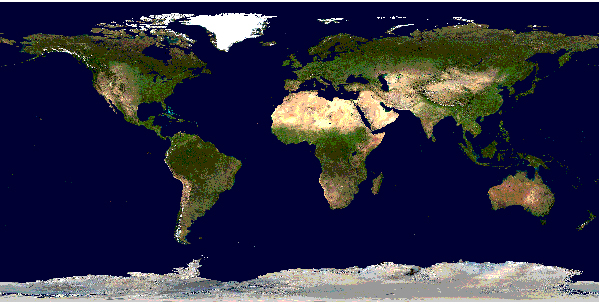
\includegraphics[width=10cm]{stepanov1.jpg}
  
  \label{Stepanov1}
\end{figure}

\end{center}


Для хранения пространственных данных большинство рассматриваемых свободно распространяемых продуктов использует СУБД PostgreSQL ~\cite{Stepanov-8}, а точнее, надстройку над СУБД ~--- PostGIS ~\cite{Stepanov-9}, позволяющую хранить в себе пространственные данные (точки, полигоны, линии и некоторые графические объекты).

\subsection*{Опыт использования в реальном проекте.}

\begin{itemize}
  \item Реализации проекта по созданию онлайн-ГИС для размещения культурных и туристических объектов Беларуси на картографической основе, доступной всем.
\begin{center}

\begin{figure}[h!]
  \centering
  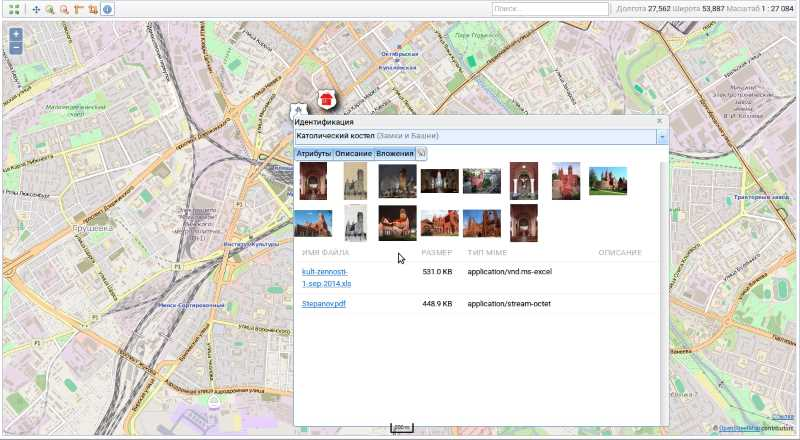
\includegraphics[width=10cm]{stepanov2.jpg}
  
  \label{Stepanov2}
\end{figure}
\begin{center}

\begin{figure}[h!]
  \centering
  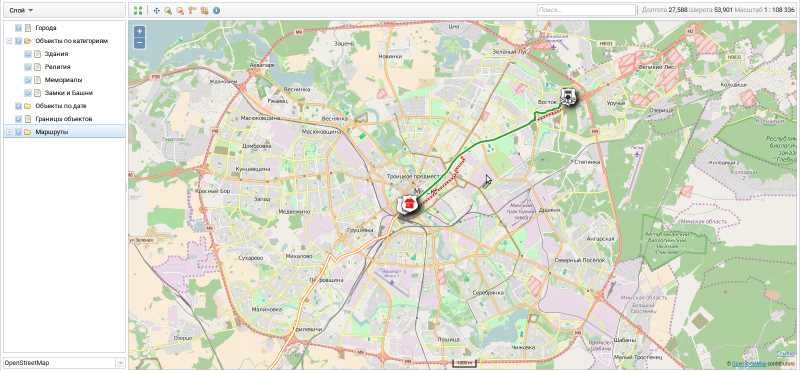
\includegraphics[width=10cm]{stepanov3.jpg}
  
  \label{Stepanov3}
\end{figure}

\end{center}

\end{center}


\end{itemize}

\begin{itemize}
  \item Отображение на картографической основе информации о работе светофоров с динамическим изменением стилистики отображаемого слоя.
  \item Отображение на картографической основе зон отношения к определенному гос. учреждению (милиция, поликлиника, \linebreak ЖЭС и т.д.v1)

\begin{center}

\begin{figure}[h!]
  \centering
  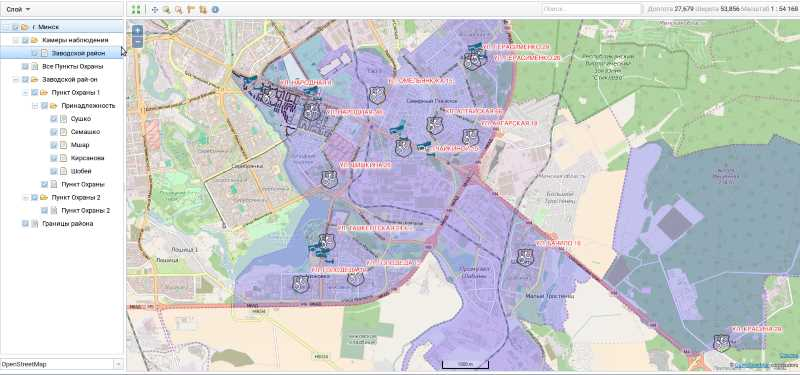
\includegraphics[width=10cm]{stepanov4.jpg}
  
  \label{Stepanov4}
\end{figure}

\end{center}

\end{itemize}

Подытожив, хочется воспользоваться цитатой из киносерии про пирата Джека Воробья:
 ~--- Да, раньше этот мир был куда больше\ldots{}
 ~--- Нет, мир остался прежним. Стало меньше содержимого.

\begin{thebibliography}{99}

\bibitem{Stepanov-1}Официальный портал продукта QGIS ~---  \url{http://qgis.org}{qgis.org}
\bibitem{Stepanov-2}Проект QGIS на гитхабе ~--- \url{https://github.com/qgis/QGIS}
\bibitem{Stepanov-3}Веб-клиент для работы с QGIS ~--- \url{https://github.com/qgis/QGIS-Web-Client}
\bibitem{Stepanov-4}Сайт продукта NEXTGISQGIS ~--- \url{http://nextgis.ru/nextgis-qgis/}
\bibitem{Stepanov-5}Реализация QGIS WEB Server ~--- \url{https://live.osgeo.org/ru/quickstart/qgis_mapserver_quickstart.html}
\bibitem{Stepanov-6}GIS-Lab ~--- неформальное сообщество специалистов в области ГИС и ДЗЗ ~--- \url{http://gis-lab.info/}
\bibitem{Stepanov-7}Ресурс картографической основы ~--- \url{http://www.openstreetmap.org}
\bibitem{Stepanov-8}СУБД ~--- \url{https://www.postgresql.org/}
\bibitem{Stepanov-9}Расширение для базы данных PostgreSQL ~---  \url{http://www.postgis.net/}
\bibitem{Stepanov-10}Проект NEXTGIS на гитхабе ~--- \url{https://github.com/nextgis}
\bibitem{Stepanov-11}Сайт продукта NEXTGIS ~--- \url{http://nextgis.ru/}
\bibitem{Stepanov-12}Проект NEXTGISWEB на гитхабе ~--- \url{https://github.com/nextgis/nextgisweb}
\bibitem{Stepanov-13}Интеграция публикации стилей слоев QGIS на NEXTGISWEB ~--- \url{https://github.com/nextgis/nextgisweb_qgis}
\end{thebibliography}

\end{document}
